\documentclass[a4paper,10pt]{book}

\usepackage[T1]{fontenc}
\usepackage[utf8]{inputenc}
%\usepackage{mathtools}
\usepackage{graphicx}
\usepackage[margin=1in]{geometry}
%\usepackage[spanish]{babel}
\usepackage[hidelinks]{hyperref}
\usepackage{fancyhdr}
\usepackage{incgraph,tikz}
\usepackage{caption}
\usepackage{subcaption}
\usepackage{amsmath} % agregado
\usepackage{amsfonts}
\usepackage{babel}
\usepackage{color}
\usepackage{listings}
\usepackage{float}
\usepackage{tikz}
\usepackage{adjustbox}
\usepackage{natbib}
\usepackage{subcaption}
\usepackage{cleveref}
\usepackage{colortbl} % agregado 
\usepackage{xcolor}
\usepackage{titlepic}

\usepackage{listings}
\lstset{ %
basicstyle=\footnotesize,       % the size of the fonts that are used for the code
numbers=none,                   % where to put the line-numbers
numberstyle=\footnotesize,      % the size of the fonts that are used for the line-numbers
stepnumber=1,                   % the step between two line-numbers. If it is 1 each line will be numbered
numbersep=10pt,                  % how far the line-numbers are from the code
backgroundcolor=\color{white},  % choose the background color. You must add \usepackage{color}
showspaces=false,               % show spaces adding particular underscores
showstringspaces=false,         % underline spaces within strings
showtabs=false,                 % show tabs within strings adding particular underscores
frame=single,           % adds a frame around the code
tabsize=4,          % sets default tabsize to 2 spaces
captionpos=b,           % sets the caption-position to bottom
breaklines=true,        % sets automatic line breaking
breakatwhitespace=false,    % sets if automatic breaks should only happen at whitespace
escapeinside={\%*}{*)}          % if you want to add a comment within your code
}

\usetikzlibrary{arrows}

\captionsetup[subfigure]{subrefformat=simple,labelformat=simple}

\renewcommand{\contentsname}{\'Indice General}
\renewcommand{\listfigurename}{\'Indice de Figuras}
\renewcommand{\listtablename}{\'Indice de Tablas}
\renewcommand{\lstlistingname}{Salida}
\renewcommand\tablename{Tabla}
\renewcommand{\figurename}{Figura}
\renewcommand\thesubfigure{(\alph{subfigure})}
\renewcommand{\baselinestretch}{1.2} 

\makeatletter
\def\verbatim{\small\@verbatim \frenchspacing\@vobeyspaces \@xverbatim}
\makeatother

\pagestyle{fancy}

\restylefloat{table}

\title{Detección de Anomalías Utilizando Autocodificadores}
\author{Autor: Matías Cisnero\\ Tutor: Dra. M. Juliana Gambini}
\date{Diciembre 2025 \\ Universidad Nacional de Hurlingham}
\titlepic{\vspace{12cm}
\includegraphics[width=0.15\textwidth]{logo.png}}

\newcommand{\comentario}[1]{\textbf{\textcolor{red}{#1}}}

\begin{document}

\maketitle


\tableofcontents
\listoffigures
\listoftables

\chapter*{Resumen}

El presente \underline{trabajo (o informe)} aborda el problema de la detección de anomalías en conjuntos de datos de salud, enfocándose en el diagnóstico temprano y la prevención de enfermedades como la diabetes. Se emplea la arquitectura de Autocodificadores (\textit{Autoencoders}), una clase de red neuronal no supervisada, para aprender una representación compacta y eficiente de los patrones de datos normales. El modelo se entrena utilizando el conjunto de datos \textbf{Diabetes Health Indicators Dataset}, donde se considera anómalo cualquier patrón que se desvía significativamente de la reconstrucción esperada. La implementación se realiza mediante la biblioteca PyTorch. Los resultados de esta investigación muestran ***. Se presenta un análisis exploratorio de los datos inicial, incluyendo la matriz de correlación y ***.

\chapter{Introducción}

\comentario{Describir el problema que se desea resolver}\\

La detección de anomalías es un campo fundamental dentro del análisis de datos, cuyo objetivo principal es la identificación de patrones que no se ajustan a un comportamiento que coincide con el de la mayoría de los registros. En el contexto de los datos de salud, una anomalía puede representar un error de medición, o una indicación temprana de una condición médica patológica, como la diabetes. Este trabajo se centra en desarrollar un sistema robusto para la detección automática de tales desviaciones. Se busca resolver la limitación de los métodos estadísticos tradicionales, los cuales a menudo no logran capturar las complejas interrelaciones no lineales presentes en conjuntos de datos de alta dimensionalidad. El problema específico que se aborda es cómo entrenar un \textbf{autocodificador} para que aprenda exclusivamente el perfil de pacientes normales o sanos a partir de un conjunto de datos que solamente incluya pacientes sanos y otro con pacientes sanos y enfermos, y cómo utilizar su error de reconstrucción para señalar con precisión qué registros se consideran anómalos.

\section{Motivación}

\comentario{Explicar porqué estudiamos este problema, para qué sirve, cuál es el impacto y en qué áreas.}\\

El diagnóstico temprano de enfermedades como la diabetes es una tarea prioritaria en la medicina moderna. En muchos casos, los datos clínicos contienen patrones sutiles que pueden pasar desapercibidos a través de métodos tradicionales de análisis. Por este motivo, resulta fundamental el desarrollo de herramientas automáticas capaces de detectar irregularidades de manera precisa y rápida.

Las redes neuronales, y en particular los autocodificadores, ofrecen un enfoque adecuado para esta tarea. Un autocodificador es un tipo de red neuronal diseñado para aprender una representación comprimida de los datos, capturando sus características más relevantes. Esta capacidad lo convierte en un candidato natural para identificar desviaciones respecto del comportamiento considerado normal.

La incorporación de este tipo de modelos en sistemas de monitoreo podría asistir a profesionales de la salud en la detección temprana de pacientes en riesgo, incluso antes de la manifestación de síntomas clínicos evidentes. Por ello, en este proyecto se emplea un autocodificador como herramienta para analizar registros de pacientes y explorar su utilidad como detector de posibles anomalías asociadas a la diabetes.


\section{Estado del Arte}

\comentario{En esta sección se realiza una descripción de algunos de los métodos más importantes existentes en la bibliografía describiendo el problema y el método utilizado por cada autor. Se cita la bibliografía.}\\

\subsection{Autoencoders for Anomaly Detection Are Unreliable}

Bouman y Heskes (2025) \cite{bouman2025unreliable} analizan críticamente el uso de autoencoders clásicos como detectores de anomalías. El trabajo sostiene que, bajo ciertas condiciones, los autoencoders pueden reconstruir correctamente ejemplos anómalos, lo cual conduce a falsos negativos incluso en casos evidentes.

\textbf{Metodología.}  

\textbf{Resultados principales.}  

\textbf{Limitaciones.}  

\textbf{Relevancia.}  

\subsection{A comprehensive study of auto-encoders for anomaly detection}

Neloy y Turgeon (2024) \cite{neloy2024study}

\subsection{Enhancing Anomaly Detection Through Latent Space Manipulation}

Walczyna et al. (2025) \cite{walczyna2025latent}

\subsection{Ensemble of Autoencoders for Anomaly Detection in Biomedical Data}

\url{https://ieeexplore.ieee.org/abstract/document/10418130}

\chapter{Materiales y Métodos}

\comentario{Describir los métodos utilizados, si corresponde.}\\

%prueba \cite{santos2025}

El método empleado en este proyecto es el \textbf{Autocodificador (\textit{Autoencoder})}. Un autocodificador es un tipo de red neuronal artificial diseñada para aprender una representación codificada de un conjunto de datos de manera no supervisada. La arquitectura se compone de dos partes principales: el \textbf{Codificador (\textit{Encoder})} y el \textbf{Decodificador (\textit{Decoder})}.

\section{Conjunto de datos y análisis exploratorio}

\comentario{Se describen los datos utilizados y de donde fueron extraídos, si corresponde. En caso de que los datos sean propios, describir como fueron tomados}\\

Para la realización de este trabajo, utilicé el conjunto de datos \textbf{Diabetes Health Indicators Dataset}, el cual se extrajo de la plataforma Kaggle (disponible en: \url{https://www.kaggle.com/datasets/alexteboul/diabetes-health-indicators-dataset}). El conjunto de datos contiene 253\,680 registros y 22 atributos numéricos relacionados con indicadores de salud, hábitos de vida y características demográficas de los participantes.

\subsection*{Atributos del conjunto de datos}

A continuación, se listan los 22 atributos clasificados según su naturaleza:

\subsubsection*{Variables binarias (0 o 1)}

\begin{itemize}
	\item \textbf{Diabetes\_012:} Variable objetivo. Toma el valor 1 si la persona tiene diagnóstico de diabetes, 0 en caso contrario.
	\item \textbf{HighBP:} Indica si la persona presenta presión arterial alta (1 = sí, 0 = no).
	\item \textbf{HighChol:} Indica si la persona tiene colesterol alto (1 = sí, 0 = no).
	\item \textbf{CholCheck:} Indica si la persona se ha realizado un chequeo de colesterol en los últimos cinco años (1 = sí, 0 = no).
	\item \textbf{Smoker:} Indica si la persona ha fumado al menos 100 cigarrillos en su vida (1 = sí, 0 = no).
	\item \textbf{Stroke:} Indica si la persona ha sufrido un accidente cerebrovascular (ACV) (1 = sí, 0 = no).
	\item \textbf{HeartDiseaseorAttack:} Indica si la persona tuvo alguna enfermedad coronaria o ataque cardíaco (1 = sí, 0 = no).
	\item \textbf{PhysActivity:} Indica si la persona realizó actividad física en los últimos 30 días (1 = sí, 0 = no).
	\item \textbf{Fruits:} Indica si la persona consume frutas al menos una vez al día (1 = sí, 0 = no).
	\item \textbf{Veggies:} Indica si la persona consume vegetales al menos una vez al día (1 = sí, 0 = no).
	\item \textbf{HvyAlcoholConsump:} Indica si la persona tiene un consumo elevado de alcohol (1 = sí, 0 = no).
	\item \textbf{AnyHealthcare:} Indica si la persona tiene algún tipo de cobertura médica (1 = sí, 0 = no).
	\item \textbf{NoDocbcCost:} Indica si la persona no pudo consultar a un médico por motivos de costo en los últimos 12 meses (1 = sí, 0 = no).
	\item \textbf{DiffWalk:} Indica si la persona tiene dificultad para caminar o subir escaleras (1 = sí, 0 = no).
	\item \textbf{Sex:} Género del participante (0 = femenino, 1 = masculino).
\end{itemize}

\subsubsection*{Variables no binarias}

\begin{itemize}
	\item \textbf{BMI:} Índice de masa corporal (Continua).
	\item \textbf{GenHlth:} Autoevaluación del estado general de salud en una escala del 1 (excelente) al 5 (malo) (Discreta, Ordinal).
	\item \textbf{MentHlth:} Número de días en los últimos 30 en los que la salud mental no fue buena (Discreta, Conteo).
	\item \textbf{PhysHlth:} Número de días en los últimos 30 en los que la salud física no fue buena (Discreta, Conteo).
	\item \textbf{Age:} Grupo etario codificado en rangos de 5 años (del 1 al 13, donde el valor 1 representa 18 a 24 años y el valor 13 representa 80 años o más) (Discreta, Ordinal).
	\item \textbf{Education:} Nivel educativo, codificado del 1 (sin educación formal o solo jardín de infantes) al 6 (graduado universitario) (Discreta, Ordinal).
	\item \textbf{Income:} Nivel de ingresos, codificado del 1 (menos de \$10.000 anuales) al 8 (más de \$75.000 anuales) (Discreta, Ordinal).
\end{itemize}

\subsection{Análisis exploratorio de datos y preprocesamiento}

Previo al entrenamiento del modelo, realicé un \textbf{análisis exploratorio de datos (EDA)}. Este proceso incluye la limpieza de datos, el manejo de valores faltantes (si los hay), la visualización de la distribución de las variables y, fundamentalmente, el cálculo y la visualización de la matriz de correlación entre todos los atributos.

Se aplicó una \textbf{estandarización} a los atributos no binarios para asegurar que todas las entradas del modelo tienen una escala comparable.

La matriz de correlación resulta crucial porque permite identificar las \textbf{dependencias lineales} entre las variables y guía las decisiones sobre el preprocesamiento de los datos, confirmando la necesidad de un modelo capaz de capturar relaciones más complejas, como el autocodificador.

\subsubsection{Distribución de la variable objetivo}

La variable objetivo, $\textit{Diabetes\_012}$, presenta la siguiente distribución, lo que evidencia un problema de \textbf{desbalance de clases} que debe ser abordado por el modelo:

\begin{table}[H]
	\centering
	\caption{Distribución de la variable objetivo \textit{Diabetes\_012}}
	\begin{tabular}{|c|c|c|}
		\hline
		\textbf{Valor} & \textbf{Porcentaje (\%)} & \textbf{Cantidad de registros} \\ \hline
		0.0 (\textit{Sin diabetes}) & 84.24 & 213\,703 \\ \hline
		2.0 (\textit{Con diabetes}) & 13.93 & 35\,346 \\ \hline
		1.0 (\textit{Prediabetes}) & 1.83 & 4\,631 \\ \hline
	\end{tabular}
	\label{tab:diabetes_012}
\end{table}

Para el caso de este trabajo, se quitaron los registros correspondientes a pacientes con prediabetes, resultando en la siguiente distribución:

\begin{table}[H]
	\centering
	\caption{Distribución de la variable objetivo \textit{Diabetes\_012} posterior al filtrado}
	\begin{tabular}{|c|c|c|}
		\hline
		\textbf{Valor} & \textbf{Porcentaje (\%)} & \textbf{Cantidad de registros} \\ \hline
		0.0 (\textit{Sin diabetes}) & 85.81 & 213\,703 \\ \hline
		1.0 (\textit{Con diabetes}) & 14.19 & 35\,346 \\ \hline
	\end{tabular}
	\label{tab:diabetes_012_filtrado}
\end{table}

El conjunto de datos contiene atributos con diferentes rangos de valores; por ejemplo, el \textbf{BMI} es continuo, mientras que \textbf{Age}, \textbf{Education} e \textbf{Income} son escalas ordinales. Esta diferencia de escalas puede afectar el rendimiento de los algoritmos de optimización (como el Descenso de Gradiente) en el autocodificador, ya que las características con rangos más grandes dominarían la función de pérdida.

Para mitigar esto, apliqué una estandarizacióna a todos los atributos no binarios. La estandarización transforma las variables para que tengan una media ($\mu$) de cero y una desviación estándar ($\sigma$) de uno, asegurando que todas las entradas al modelo tienen una escala comparable. Se realiza de la siguiente manera:

\[
z = \frac{x - \mu}{\sigma}
\]

donde $x$ es el valor original del atributo, $\mu$ es su media y $\sigma$ es su desviación estándar.



Calculo la matriz de correlación ($\rho$), la cual mide el grado de asociación lineal entre cada par de atributos del conjunto de datos. Se calcula de la siguiente manera:

\[
\rho(X, Y) = \frac{Cov(X, Y)}{s_x s_y}
\]

Donde $Cov(X, Y)$ representa la covarianza entre $X$ e $Y$, y $s_x$, $s_y$ son sus desviaciones estándar. La covarianza se define como:

\[
Cov(X, Y) = \frac{1}{n} \sum_{i=1}^n (x_i - \bar{x})(y_i - \bar{y})
\]

A continuación se muestra la matriz de correlación calculada para los principales indicadores de salud del dataset:

\begin{figure}[H]
	\centering
	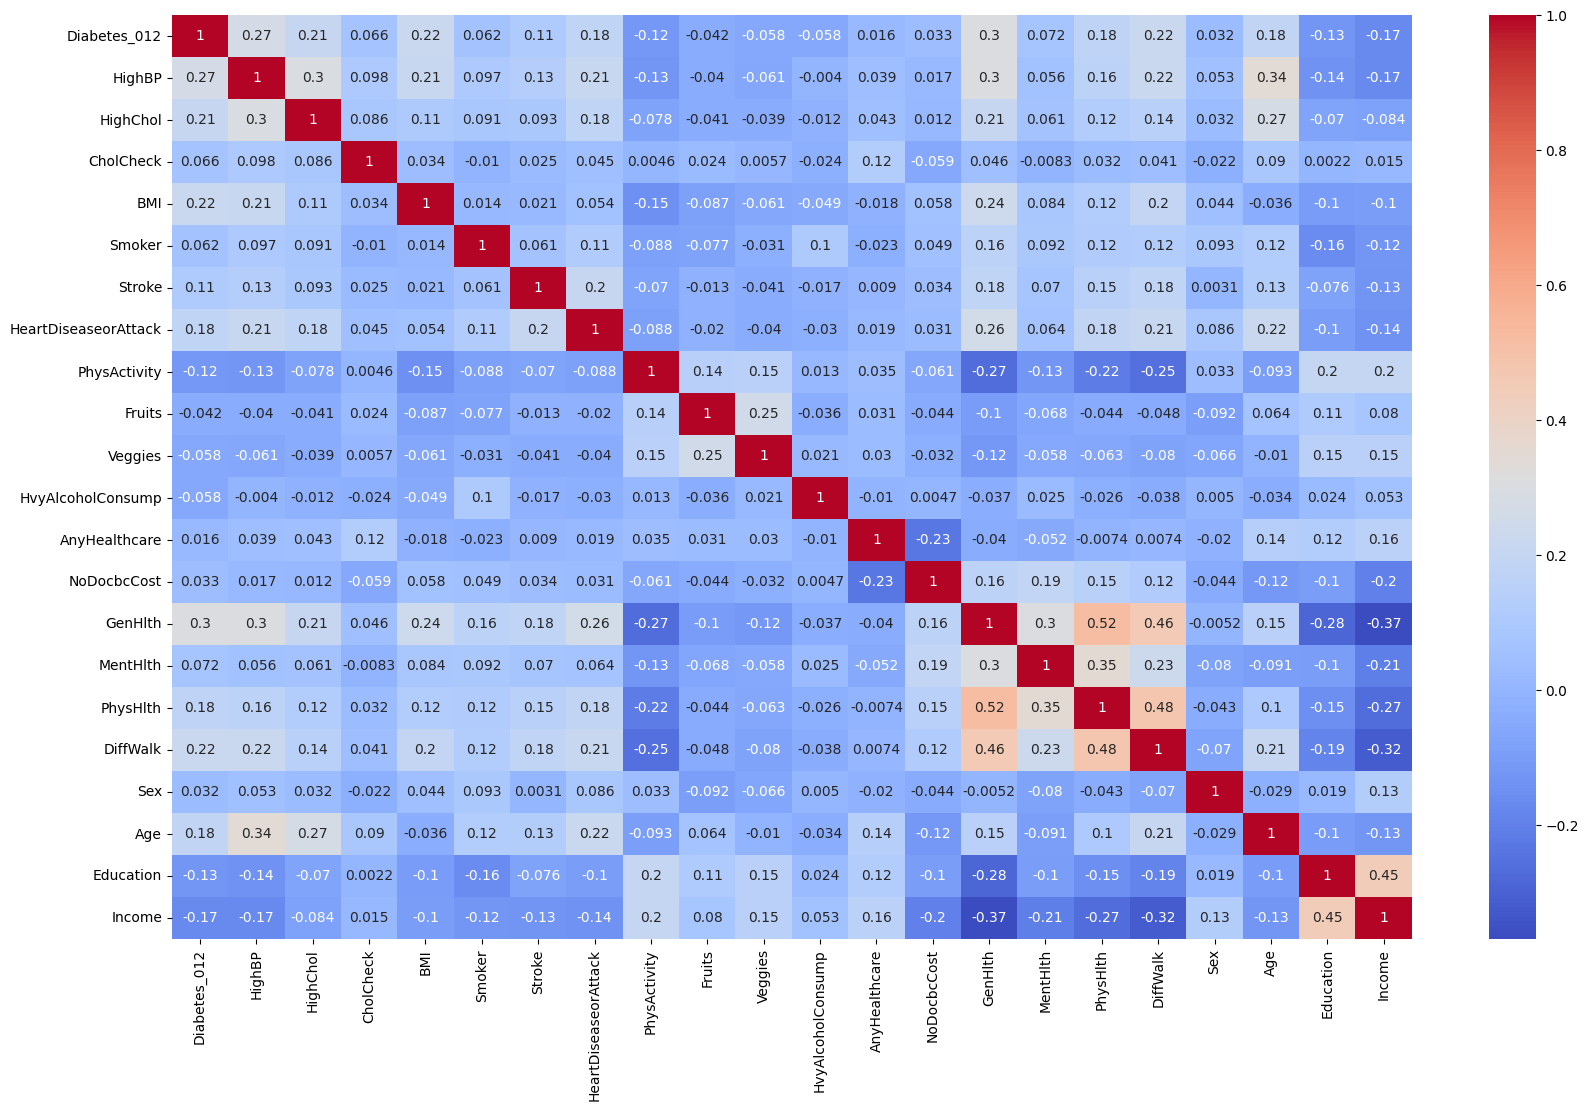
\includegraphics[width=0.8\textwidth]{corr_matrix.png}
	\caption{Matriz de correlación entre los atributos del conjunto de datos.}
	\label{fig:corr_matrix}
\end{figure}

Para realizar el entrenamiento del autocodificador usé 4 conjuntos, los cuales poseen distintas proporciones de datos atípicos, esto lo realizo con el fin de evaluar la robustez del modelo ante estos. Cada conjunto de entrenamiento mantuvo un \textbf{total de 70\,692 registros}.

\begin{table}[H]
	\centering
	\caption{Conjuntos de datos creados para evaluar la resistencia a anomalías}
	\begin{tabular}{|c|c|c|c|c|}
		\hline
		\textbf{ID} & \textbf{Proporción Anómalos} & \textbf{Proporción Normales} & \textbf{Registros Anómalos} & \textbf{Registros Normales} \\
		& (\% Total) & (\% Total) & (Positivos) & (Negativos) \\ \hline
		A & 0\% & 100\% & 0 & 70\,692 \\ \hline
		B & 10\% & 90\% & 7\,069 & 63\,623 \\ \hline
		C & 25\% & 75\% & 17\,673 & 53\,019 \\ \hline
		D & 50\% & 50\% & 35\,346 & 35\,346 \\ \hline
	\end{tabular}
	\label{tab:resistencia_anomalias}
\end{table}

Estos conjuntos representan la proporción de contaminación introducida en el dataset de entrenamiento para simular escenarios donde la pureza de los datos normales no está garantizada.

Para cada conjunto realicé una división en entrenamiento y prueba, manteniendo la proporción de normales y anomalías correspondiente a cada caso. El conjunto de entrenamiento se obtuvo tomando el 80\% de las muestras del conjunto original, mientras que el 20\% restante se utilizó como conjunto de prueba. De esta manera, tanto la distribución de clases como las diferentes proporciones de contaminación se mantienen consistentes en ambos subconjuntos, permitiendo evaluar el desempeño del modelo bajo escenarios comparables.

\section{Descripción de los métodos}

Él método empleado en este proyecto es un autocodificador, un tipo de perceptrón multicapa caracterizado por su estructura simétrica respecto a la capa latente y por tener la misma dimensión en la entrada ($d$) y en la salida. Aunque suele decirse que el aprendizaje en este modelo es no supervisado, en realidad sí es supervisado, ya que la salida esperada ($Y$) es la propia entrada ($X$).

En esta arquitectura, el \textbf{codificador} comprime la entrada en una representación ubicada en la \textbf{capa latente}, que es la capa oculta central y cuya dimensión ($k$) suele ser menor que la de la entrada ($k < d$). Esta capa contiene la representación comprimida de los datos. Luego, el \textbf{decodificador}, que constituye la segunda mitad de la red, reconstruye la salida a partir de esa representación latente.

La arquitectura general de un autocodificador puede representarse de manera esquemática como se muestra en la Figura~\ref{fig:arquitectura}. En ella se observa las distintas capas del modelo, desde la entrada hasta la salida.

\begin{figure}[H]
	\centering
	
\includegraphics[width=0.6\linewidth]{arquitectura}
	\caption{Arquitectura de un autocodificador: la entrada $X$ es procesada por el codificador hasta obtener la representación latente $Z$, a partir de la cual el decodificador reconstruye la salida $Y$.}
	\label{fig:arquitectura}
\end{figure}

Como función de activación en mi autocodificador utilizo \text{GELU} debido a sus ventajas frente a la comúnmente empleada \text{ReLU}. Entre ellas se destacan: una superficie de pérdida más suave que facilita un entrenamiento más estable y rápido, la ausencia del problema de "neuronas muertas" propio de ReLU, y una mayor capacidad de modelar relaciones no lineales gracias a su naturaleza probabilística basada en la distribución normal.

La función GELU(x) está definida por:
\[
\text{GELU}(x) = 0.5\,x\left(1 + \tanh\!\left(\sqrt{\frac{2}{\pi}}\left(x + 0.044715x^{3}\right)\right)\right)
\]

La función ReLU(x) se define como:
\[
\text{ReLU}(x) = \max(0, x)
\]

Como se muestra en la Figura~\ref{fig:relugelu}, al graficar ambas funciones se puede apreciar la suavidad de \text{GELU} al aproximarse a 0, en contraste con el comportamiento abrupto de \text{ReLU}.

\begin{figure}[H]
	\centering
	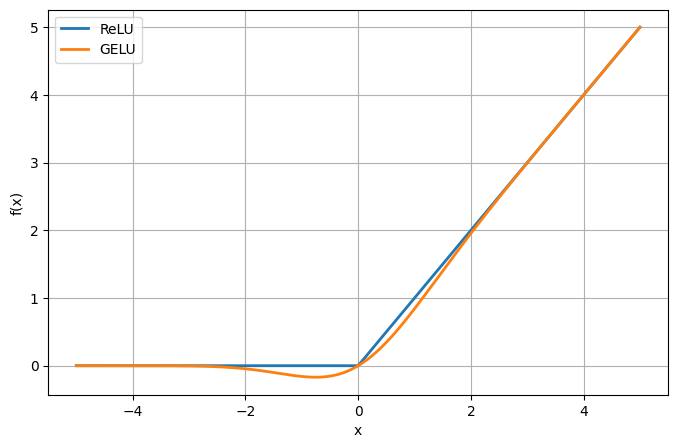
\includegraphics[width=0.6\linewidth]{relu_gelu}
	\caption{Comparación entre las funciones de activación ReLU y GELU. Se observa que GELU presenta una transición suave alrededor de cero, lo que evita discontinuidades y favorece un entrenamiento más estable en modelos neuronales.}
	\label{fig:relugelu}
\end{figure}

A partir de esta arquitectura, el autocodificador puede emplearse como un método de \textbf{detección de anomalías}. Para ello, el modelo se entrena exclusivamente con la clase que representa el comportamiento normal, es decir, pacientes sin diabetes. Debido a que aprende a reconstruir adecuadamente este tipo de patrones, cuando recibe un dato $t$ perteneciente a la misma distribución, se espera que el error de reconstrucción $||t' - t||$ sea pequeño.

En contraste, si se presenta un dato atípico $t^{*}$, correspondiente a un paciente con diabetes el modelo no logra reconstruirlo con la misma fidelidad, generando así un error significativamente mayor. Este comportamiento permite establecer un criterio simple y efectivo para la detección de anomalías: un dato se clasifica como anómalo si su error de reconstrucción supera un umbral $\epsilon$ predefinido. Formalmente:

\[
||t^{*} - t^{\prime *}|| > \epsilon
\]

donde $t^{\prime *}$ es la reconstrucción producida por la red a partir del dato $t^{*}$. Si la desigualdad se cumple, el dato se considera \emph{anómalo}; de lo contrario, se clasifica como \emph{normal}.

El valor del umbral $\epsilon$ se determinó de manera empírica a partir del conjunto de datos normales utilizado durante el entrenamiento. En particular, se calculó como la \textbf{media del error de reconstrucción}:

\[
\epsilon = \text{media}\!\left( \lVert t'_i - t_i \rVert \right)
\]

donde $t_i$ corresponde a cada muestra normal y $t'_i$ a su respectiva reconstrucción generada por el modelo. Este valor promedio proporciona un límite representativo del comportamiento esperado en datos no anómalos, permitiendo distinguir de forma efectiva aquellos casos cuyo error excede significativamente lo aprendido por la red.

\subsection{Métricas de evaluación del modelo}

Para evaluar el rendimiento del autocodificador en la tarea de detección de anomalías, se recurre a la \textbf{matriz de confusión}, la cual resume la relación entre las predicciones del modelo y las etiquetas reales. En este contexto, cada instancia se clasifica como \emph{normal} o \emph{anómala} según su error de reconstrucción $||t' - t||$ comparado con un umbral $\epsilon$.

A partir de este criterio, se definen los siguientes casos:

\begin{itemize}
	\item \textbf{Verdaderos Positivos (TP)}: Casos \emph{anómalos} (personas con diabetes) cuyo error de reconstrucción satisface $||t' - t|| > \epsilon$.
	
	\item \textbf{Falsos Negativos (FN)}: Casos \emph{anómalos} (con diabetes) pero cuyo error cumple $||t' - t|| \le \epsilon$, es decir, el modelo no detectó la anomalía.
	
	\item \textbf{Verdaderos Negativos (TN)}: Casos \emph{normales} (sin diabetes) cuyo error satisface $||t' - t|| \le \epsilon$.
	
	\item \textbf{Falsos Positivos (FP)}: Casos \emph{normales} (sin diabetes) cuyo error satisface $||t' - t|| > \epsilon$, siendo incorrectamente clasificados como anómalos.
\end{itemize}

Luego, con estos casos, se construye la siguiente matriz de confusión:

\begin{table}[H]
	\centering
	\renewcommand{\arraystretch}{1.8}
	\begin{tabular}{c|c|c|}
		\multicolumn{1}{c}{} &
		\multicolumn{2}{c}{\textbf{Predicción}} \\
		\multicolumn{1}{c}{} &
		\textbf{Anómalo} & \textbf{Normal} \\ \hline
		\textbf{Real: Anómalo} &
		\cellcolor{green!25}\textbf{Verdadero Positivo (TP)} &
		\cellcolor{red!25}\textbf{Falso Negativo (FN)} \\ \hline
		\textbf{Real: Normal} &
		\cellcolor{red!25}\textbf{Falso Positivo (FP)} &
		\cellcolor{green!25}\textbf{Verdadero Negativo (TN)} \\ \hline
	\end{tabular}
	\caption{Matriz de confusión. La diagonal verde representa predicciones correctas, mientras que las celdas rojas corresponden a errores de clasificación.}
\end{table}

A partir de la matriz de confusión, las métricas empleadas para cuantificar el rendimiento del modelo se definen como:

\[
\text{Accuracy} =
\frac{\text{TP} + \text{TN}}
{\text{TP} + \text{FP} + \text{TN} + \text{FN}}
\]

\[
\text{Precision} =
\frac{\text{TP}}
{\text{TP} + \text{FP}}
\]

\[
\text{Recall} =
\frac{\text{TP}}
{\text{TP} + \text{FN}}
\]

\[
\text{Specificity} =
\frac{\text{TN}}
{\text{TN} + \text{FP}}
\]

\[
\text{Balanced Accuracy} =
\frac{\text{Recall} + \text{Specificity}}{2}
\]

\[
\text{F1\_Score} =
\frac{2\,\text{TP}}
{2\,\text{TP} + \text{FP} + \text{FN}}
\]

En mí caso, resulta especialmente importante maximizar las métricas de \textbf{Recall} y \textbf{Precision}. Un alto \textit{Recall} asegura que la mayoría de los casos anómalos sean detectados (minimizando falsos negativos), mientras que una alta \textit{Precision} garantiza que las instancias señaladas como anómalas realmente lo sean (reduciendo falsos positivos).

\chapter{Resultados}

\comentario{Mostrar los resultados obtenidos utilizando gráficos, tablas, figuras, etc}

\begin{table}[H]
	\centering
	\caption{Métricas de rendimiento del modelo evaluado en diferentes proporciones de datos anómalos en el entrenamiento}
	\begin{tabular}{|l|c|c|c|c|}
		\hline
		\textbf{Métrica} & \textbf{Conjunto 0} & \textbf{Conjunto 1} & \textbf{Conjunto 2} & \textbf{Conjunto 3} \\
		& (0\% Anómalos) & (10\% Anómalos) & (25\% Anómalos) & (50\% Anómalos) \\ \hline
		\textit{Accuracy} & 0.5362 & - & - & - \\ \hline
		\textit{Precision} & 0.2638 & - & - & - \\ \hline
		\textit{Recall} & 0.7484 & - & - & - \\ \hline
		\textit{Specificity} & 0.4838 & - & - & - \\ \hline
		\textit{Balanced Accuracy} & 0.6161 & - & - & - \\ \hline
		\textit{F1\_Score} & 0.3901 & - & - & - \\ \hline
	\end{tabular}
	\label{tab:metricas_resistencia_anomalias}
\end{table}

\begin{figure}[H]
	\centering
	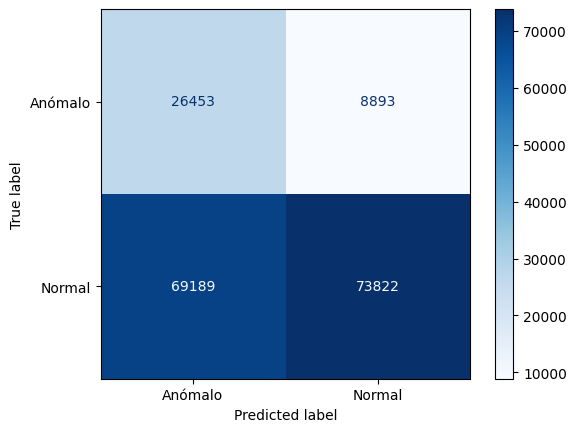
\includegraphics[width=0.7\textwidth]{matriz_conf_abs.png}
	\caption{Matriz de confusión en valores absolutos.}
	\label{fig:matriz_conf_abs}
\end{figure}

\begin{figure}[H]
	\centering
	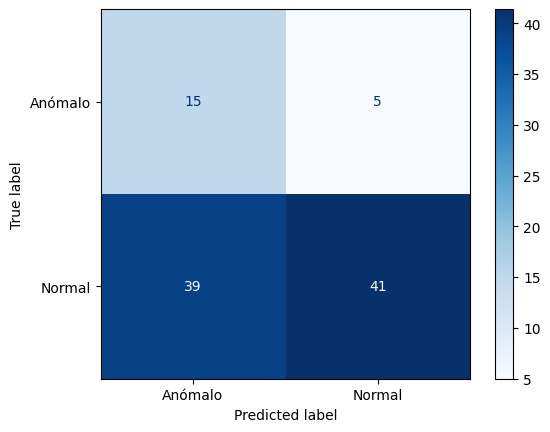
\includegraphics[width=0.7\textwidth]{matriz_conf_pct.png}
	\caption{Matriz de confusión en valores porcentuales.}
	\label{fig:matriz_conf_pct}
\end{figure}


\chapter{Conclusiones}

\comentario{Explicar que aprendimos con la realización de este trabajo. Qué nos muestran los resultados.}

\bibliographystyle{plain}
\bibliography{References}

\end{document}
